\textcolor{blue}{Suggest merging the architecure and correlation subsections.
Start with a discussion of the problem (1) layers each maintain state that
idenfifies internal state, (2) Roots need to identify the state change
events that are triggered by a specific event's processing.  Change the figure
to reflect this requirement and discuss how this architecture allow
Roots to correlate state change events with individual request processing.}


The key intuition behind Roots is that
the cloud platform can aid the developer detect anomalies in deployed applications.
The cloud platform has full visibility into all the activities that occur in various layers of the cloud,
including all invocations of the PaaS kernel services. Therefore
it can automatically collect data regarding events that are related to application request processing. 
The cloud platform can then analyze the collected data offline (but in near realtime) to detect 
performance anomalies and identify root causes.

We argue that data collection can be implemented efficiently in the cloud platform so as to not
introduce a significant overhead to deployed applications.
Moreover, data collection can be always active in the cloud thus relieving the application developers
from having to instrument their code, or setting up external monitoring.
The data analysis can benefit from the vast amount of compute
resources available in the cloud platform. The offline processing ensures that application request
processing is not impacted by monitoring, and the near realtime analysis ensures that developers
and other interested parties are notified of performance anomalies urgently. 

\subsubsection{Data Collection and Storage}
\begin{figure}
\centering
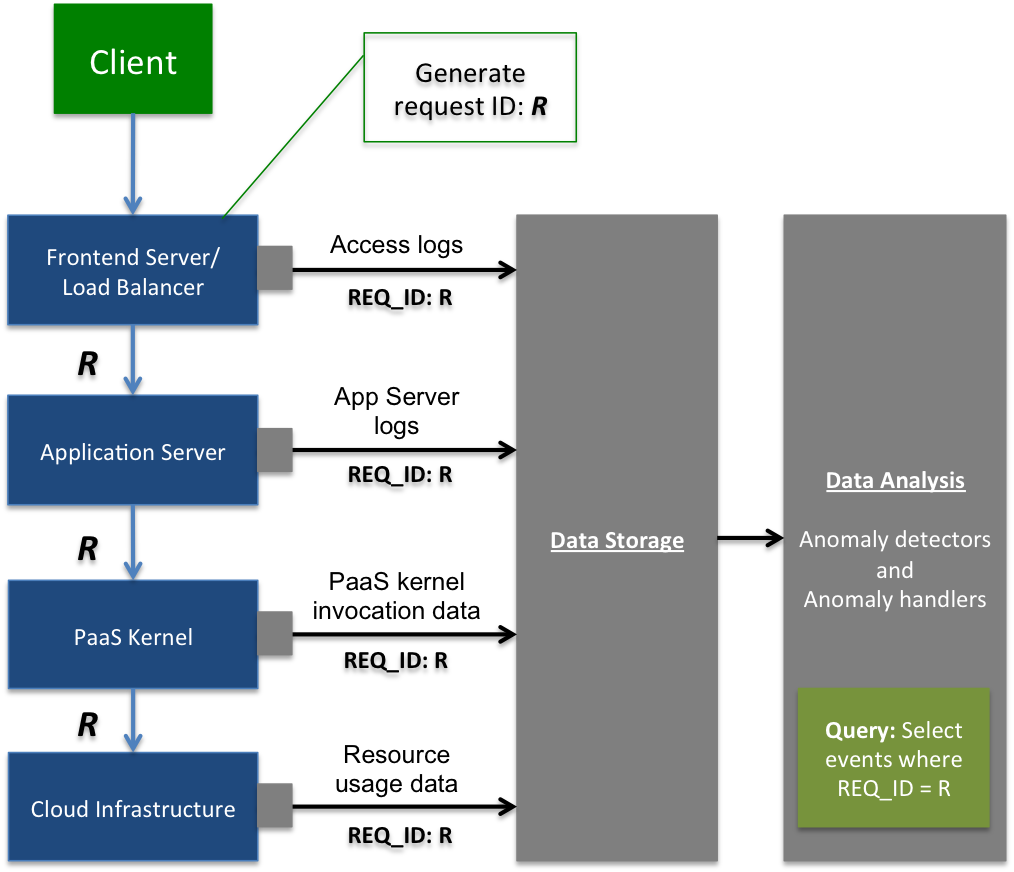
\includegraphics[scale=0.5]{apm_architecture}
\caption{Roots APM architecture.}
\label{fig:apm_architecture}
\end{figure}

Figure~\ref{fig:apm_architecture} illustrates the high-level architecture of the proposed APM, and how 
it fits into the PaaS cloud stack. APM components are shown in grey, with their interactions indicated
by the black lines. The small grey boxes attached to the PaaS components represent the sensors and
agents used to instrument the cloud platform for data collection purposes. Note that the APM collects
data from all layers in the PaaS stack (i.e. full stack monitoring).

From the front-end and load balancing layer we gather all information related to incoming application
requests. A big part of this is scraping the HTTP server access logs, which indicate request timestamps,
source and destination addressing information, response time (latency) and other HTTP message
parameters. This information is readily available for harvesting in most technologies used as front-end
servers (e.g. Apache HTTPD, Nginx). Additionally we may also collect information pertaining to active
connections, invalid access attempts and other errors.

From the application server layer we collect basic application logs as well as any other
metrics that can be easily collected from the application runtime. This may include some process level
metrics indicating the resource usage of the individual application instances. Additionally Roots
employs a set of per-application benchmarking processes, that periodically probes applications
to measure their performance. These are lightweight, stateless processes managed by the Roots framework.
Data collected by these processes will also be sent to data storage component, and will be available
for analysis as per-application timeseries data.

At the PaaS kernel layer we employ instrumentation to record information regarding all kernel invocations
made by the applications. This instrumentation must be applied carefully as to not introduce a noticeable
overhead to the application execution. For each PaaS kernel invocation, we can capture the 
following parameters.
\begin{itemize}
\item Source application making the kernel invocation
\item Timestamp
\item A sequence number indicating the order of PaaS kernel invocations within an application request
\item Target kernel service and operation
\item Execution time of the invocation
\item Request size, hash and other parameters
\end{itemize}
Collecting this PaaS kernel invocation details enables tracing the execution of application 
requests, without the need for instrumenting application code, which we believe is a feature 
unique to Roots. 

Finally, at the lowest infrastructure level, we can collect information related to virtual machines, containers
and their resource usage. We can also gather metrics on network usage by individual components which
might be useful in a number of traffic engineering use cases. Where appropriate we can also scrape
hypervisor and container manager logs to get an idea of how resources are allocated and released over
time.

To avoid introducing delays to the application request processing flow, we implement
all Roots data collecting agents as asynchronous tasks. That is, none of them would
suspend application request processing to report data to the data storage components.
We make sure that all expensive I/O tasks related to data collection and storage is
executed out of the request processing flow.
In particular, all data is collected into log files or memory buffers that are local to the components being
monitored. This locally collected (or buffered) data will be periodically sent
to the data storage components of Roots using separate background tasks and batch communication
operations. Also special care is taken to isolate the activities in the cloud from potential
faults in the Roots data collection or storage components.

The Roots data storage is a database that supports persistently storing monitoring data, and running
queries on them.  
Cloud providers have the freedom to implement this component in any way they see fit, as long
as it scales to the number of applications deployed in the cloud platform. Most data retrieval queries executed
by Roots use application and time intervals as indices. Therefore a database that can index monitoring
data by application, and then organize records by timestamp will greatly improve the query performance.
It is also acceptable to remove old monitoring data to make room for more recent events, since Roots
is performing anomaly detection using the most recent data in near realtime.

\subsubsection{Cross-layer Data Correlation}
Roots must be able to correlate data records collected at different layers of the PaaS. For example consider
the execution of a single application request. This single event results in following data records at
different layers of the cloud, which will be collected and stored by the APM as separate entities.

\begin{itemize}
\item A front-end server access log entry
\item Zero or more application log entries
\item Zero or more PaaS kernel invocation records
\end{itemize}

We require a mechanism to tie these disparate records together, so the data analysis components can easily
aggregate the related information. For instance, we must be able to retrieve via an
aggregation query, all PaaS kernel invocations made by a specific application request.

To facilitate this requirement we propose that the front-end server tags all incoming application requests 
with unique identifiers.
This request identifier can be attached to HTTP requests as a header which is visible to all components 
internal to the PaaS cloud. All data collecting agents can then be configured to record the request identifiers
whenever recording an event. At the data analysis components Roots can aggregate the data by request identifiers
to efficiently group the related records.

\subsubsection{Data Analysis}

Roots data analysis component uses two basic abstractions: \textit{anomaly detectors} 
and \textit{anomaly handlers}.
\textit{Anomaly detectors} are processes that periodically analyze the data collected for
each deployed application. Roots supports multiple detector implementations, where each implementation
uses a different statistical method to look for performance anomalies. Detectors are configured
at application level making is possible for different applications to use different anomaly 
detectors. Roots also supports multiple concurrent anomaly detectors on the same application, which can be used
to evaluate the efficiency of different detection strategies for any given application. Each
anomaly detector has an execution schedule (e.g. run every 60 seconds), and a sliding window 
(e.g. from 10 minutes ago to now)
associated with it. The boundaries of the window determines the time range
of the data processed by the detector at any round of execution. Window is updated 
after each round of execution. Our anomaly detector abstraction is general
enough to support detecting a wide range of anomalies. However, in our work we
mainly focus on anomaly detectors that check for violations of performance SLOs.

When an anomaly detector finds an anomaly in application performance, it sends an event
to a collection of \textit{anomaly handlers}. The event encapsulates a unique anomaly identifier, 
timestamp, application identifier and the source detector's sliding window that correspond to the
anomaly. Anomaly handlers are configured globally (i.e. each handler
receives events from all detectors), but each handler can can be programmed to handle only
certain types of events. Furthermore, they can fire their own events, which are also delivered to
all the listening anomaly handlers. Similar to detectors, Roots supports multiple anomaly handler
implementations -- one for logging anomalies, one for sending alert emails, one
for updating a dashboard etc. Additionally, Roots provides two special anomaly handler
implementations: a workload change analyzer, and a bottleneck identifier.

The ability of anomaly handlers to fire their own events, coupled with their support
for responding to a filtered subset of incoming events enables constructing
elaborate event flows with sophisticated logic. For example, the workload
change analyzer can run some analysis upon receiving an anomaly event
from any anomaly detector. If an anomaly cannot be associated with a workload
change, it can fire a different type of event. The bottleneck identifier, can
be programmed to only execute its analysis upon receiving this second type of event.
This way we perform the workload change analysis first, and perform the
systemwide bottleneck identification only when it is required to do so.

Both the anomaly detectors and anomaly handlers work with fix-sized sliding windows.
They can discard any old data as the sliding window moves along the time line.
Therefore the amount of state information these entities must keep in memory has
a strict upper bound. 
The extensibility of Roots is primarily achieved through the abstractions of anomaly
detectors and handlers. Roots makes it simple to implement new detectors and handlers,
and plug them into the system. Both the detectors and the handlers are executed
as lightweight processes that do not interfere with the rest of the processes in
the cloud platform. Failures in detectors and handlers have no impact
on the cloud platform or the deployed applications.

\subsubsection{Roots Process Management}
\begin{figure}
\centering
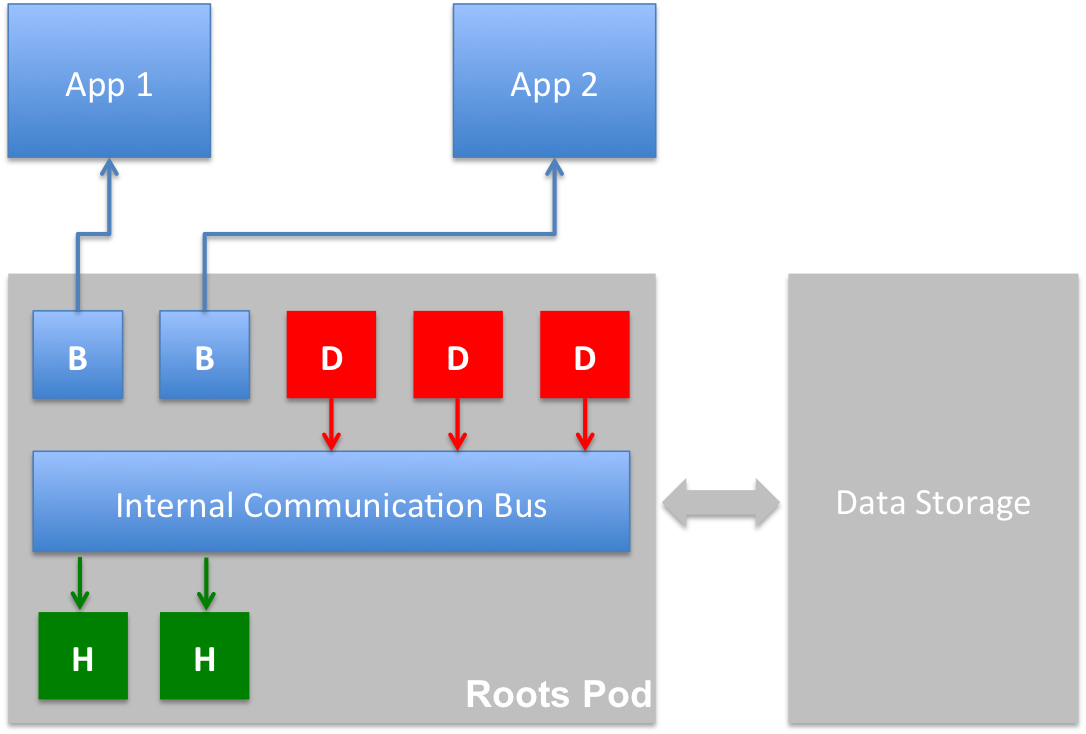
\includegraphics[scale=0.5]{roots_pod}
\caption{Anatomy of a Roots pod.}
\label{fig:roots_pod}
\end{figure}
Most data collection activities in Roots can be treated as passive -- i.e. they
happen automatically as the applications receive and process requests in the cloud
platform. They do not require explicit scheduling or management. In contrast,
application benchmarking and data analysis are active processes that require
explicit scheduling and management.  This is achieved by grouping benchmarking
and data analysis processes into units called Roots pods. 

Each Roots pod is responsible for starting and maintaining a preconfigured set of
benchmarkers and data analysis processes (i.e. anomaly detectors and handlers). 
Each of these processes are light enough, so as to pack a large number of them
into a single pod. Pods are self-contained entities, and there is no inter-communication
between pods. Processes in a pod can efficiently communicate with each other 
(using shared memory), and call out to the Roots data storage to retrieve 
collected performance data for analysis. This enables starting and stopping 
Roots pods with minimal impact on the overall monitoring system. Furthermore, pods
can be replicated for high availability, and application load can be distributed
among multiple pods for scalability.

Figure~\ref{fig:roots_pod} illustrates a Roots pod monitoring two applications.
It consists of two benchmarking processes, three anomaly detectors and 
two anomaly handlers. The anomaly detectors and handlers communicate
using an internal communication bus, so that events triggered by one anomaly
detector flow into all handlers. 

To automate the process of managing pods, they can be tied into the core
process management framework of the PaaS cloud. That way whenever the cloud
platform initializes, a collection of pods can be started automatically.
Application deployment process of the PaaS cloud can be easily augmented
to register each new application with one of the available pods, so that the
benchmarkers and anomaly detectors can start running on the application.
Moreover, pods can be moved around or restarted as needed in response
to errors and autoscaling events that occur in the cloud platform.
